\documentclass[11pt]{article}

\usepackage{fullpage}
\parindent=0in


%------------------------------------------------------------------
% PROBLEM, PART, AND POINT COUNTING...

% Create the problem number counter.  Initialize to zero.
\newcounter{problemnum}

% Specify that problems should be labeled with arabic numerals.
\renewcommand{\theproblemnum}{\arabic{problemnum}}


% Create the part-within-a-problem counter, "within" the problem counter.
% This counter resets to zero automatically every time the PROBLEMNUM counter
% is incremented.
\newcounter{partnum}[problemnum]

% Specify that parts should be labeled with lowercase letters.
\renewcommand{\thepartnum}{\alph{partnum}}

% Make a counter to keep track of total points assigned to problems...
\newcounter{totalpoints}

% Make counters to keep track of points for parts...
\newcounter{curprobpts}		% Points assigned for the problem as a whole.
\newcounter{totalparts}		% Total points assigned to the various parts.

% Make a counter to keep track of the number of points on each page...
\newcounter{pagepoints}
% This counter is reset each time a page is printed.

% This "program" keeps track of how many points appear on each page, so that
% the total can be printed on the page itself.  Points are added to the total
% for a page when the PART (not the problem) they are assigned to is specified.
% When a problem without parts appears, the PAGEPOINTS are incremented directly
% from the problem as a whole (CURPROBPTS).


%---------------------------------------------------------------------------


% The \problem environment first checks the information about the previous
% problem.  If no parts appeared (or if they were all assigned zero points,
% then it increments TOTALPOINTS directly from CURPROBPTS, the points assigned
% to the last problem as a whole.  If the last problem did contain parts, it
% checks to make sure that their point values total up to the correct sum.
% It then puts the problem number on the page, along with the points assigned
% to it.

\newenvironment{problem}[1]{
% STATEMENTS TO BE EXECUTED WHEN A NEW PROBLEM IS BEGUN:
%
% Increment the problem number counter, and set the current \ref value to that
% number.
\refstepcounter{problemnum}
%
% Add some vspace to separate from the last problem.
\vspace{0.15in} \par
%
\setcounter{curprobpts}{#1} \setcounter{totalparts}{0}	% Reset counters.
%
% Now put in the "announcement" on the page.
{\Large \bf \theproblemnum. \normalsize ({\it \arabic{curprobpts} point\null\ifnum \value{curprobpts} = 1\else s\fi}\/)}
}{
% STATEMENTS TO BE EXECUTED WHEN AN OLD PROBLEM IS ENDED:
%
% If no parts to problem, then increment TOTALPOINTS and PAGEPOINTS for the
% entire problem at once.
\ifnum \value{totalparts} = 0
	\addtocounter{totalpoints}{\value{curprobpts}}	% Add pts to total.
	\addtocounter{pagepoints}{\value{curprobpts}}	% Add pts to page total.
%
% If there were parts for the problem, then check to make sure they total up
% to the same number of points that the problem is worth. Issue a warning
% if not.
\else \ifnum \value{totalparts} = \value{curprobpts}
	\else \typeout{}
	\typeout{!!!!!!!   POINT ACCOUNTING ERROR   !!!!!!!!}
	\typeout{PROBLEM [\theproblemnum] WAS ALLOCATED \arabic{curprobpts} POINTS,}
	\typeout{BUT CONTAINS PARTS TOTALLING \arabic{totalparts} POINTS!}
	\typeout{}
	\fi
\fi
}


%---------------------------------------------------------------------------


% The \newpart command increments the part counter and displays an appropriate
% lowercase letter to mark the part.  It adds points to the point counter
% immediately.  If 0 points are specified, no point announcement is made.
% Otherwise, the announcement is in scriptsize italics.

\newcommand{\newpart}[1]
{
\refstepcounter{partnum}	% Set the current \ref value to the part number.
%\hspace{0.25in}		% Indent the part by a quarter inch.
%
% If points are to be printed for this problem (signaled by point value > 0),
% then put them in in scriptsize italics.
\ifnum #1 > 0
	\makebox[0.25in][l]{{\bf \thepartnum.} {\bf ({\it #1 pt\ifnum #1 = 1\else s\fi\/}) \,\,}}
\else
	\makebox[0.25in][l]{({\bf \thepartnum})}
\fi
%
\hspace{0.1in}		% Lead the material away from the part "number".
%
\addtocounter{totalparts}{#1}	% Add points to totalparts for this problem.
\addtocounter{pagepoints}{#1}	% Add points to total for this page.
\addtocounter{totalpoints}{#1}	% Add points to total for entire test.
}


%---------------------------------------------------------------------------



% Just in case you want to skip some numbers in your test...

\newcommand{\skipproblem}[1]{\addtocounter{problemnum}{#1}}



%---------------------------------------------------------------------------


% The \showpoints command simply gives a count of the total points read in up to
% the location at which the command is placed.  Typically, one places one
% \showpoints command at the end of the latex file, just prior to the
% \end{document} command.  It can appear elsewhere, however.

\newcommand{\showpoints}
{
\typeout{}
\typeout{====> A TOTAL OF \arabic{totalpoints} POINTS WERE READ.}
\typeout{}
}


%---------------------------------------------------------------------------



\usepackage{graphicx}
\graphicspath{ {./report_images/} }
\usepackage[english]{babel}
\usepackage[latin1]{inputenc}
\usepackage{times}
\usepackage[T1]{fontenc}
\usepackage{inconsolata}
\usepackage{amsmath}
\usepackage{amssymb}
\usepackage{hyperref}
\usepackage{color}
\usepackage{caption}
\usepackage{subcaption}
\usepackage{listings}

\newcommand{\argmax}{\mathop{\arg\max}}
\newcommand{\deriv}[1]{\frac{\partial}{\partial {#1}} }
\newcommand{\dsep}{\mbox{dsep}}
\newcommand{\Pa}{\mathop{Pa}}
\newcommand{\ND}{\mbox{ND}}
\newcommand{\De}{\mbox{De}}
\newcommand{\Ch}{\mbox{Ch}}
\newcommand{\graphG}{{\mathcal{G}}}
\newcommand{\graphH}{{\mathcal{H}}}
\newcommand{\setA}{\mathcal{A}}
\newcommand{\setB}{\mathcal{B}}
\newcommand{\setS}{\mathcal{S}}
\newcommand{\setV}{\mathcal{V}}
\DeclareMathOperator*{\union}{\bigcup}
\DeclareMathOperator*{\intersection}{\bigcap}
\DeclareMathOperator*{\Val}{Val}
\newcommand{\mbf}[1]{{\mathbf{#1}}}
\newcommand{\eq}{\!=\!}

\DeclareMathOperator*{\argmin}{arg\,min}
\DeclareMathOperator*{\sign}{sign}


\begin{document}

{\centering
  \rule{6.3in}{2pt}
  \vspace{1em}
  {\Large
    CS689: Machine Learning - Fall 2020\\
    Homework 3\\
  }
  \vspace{1em}
  Submitted by Amit Gopal Hattimare \\
  \vspace{0.1em}
  \rule{6.3in}{1.5pt}
}
\vspace{1pc}

\textbf{1.a.}
The saddle point equation is:
$$
	\min_{\mbf{w}}\max_{\alpha_{1:N}} \frac{\lambda}{2} \Vert\mbf{w}\Vert_2^2 - \sum_{n=1}^{N}(\alpha_n y_n \mbf{x}_n \mbf{w} - H(\alpha_n)) \quad \mbox{s.t.} \quad \forall n \;\; \alpha_i \in [0, 1]  
$$
We can swap the $\min$ and $\max$ operations and then take derivative w.r.t $\mbf{w}$ to find the minimum $\mbf{w}$ parameters. Our modified saddle point equation is:
\begin{equation}
	\max_{\alpha_{1:N}} \min_{\mbf{w}} \frac{\lambda}{2} \Vert\mbf{w}\Vert_2^2 - \sum_{n=1}^{N}(\alpha_n y_n \mbf{x}_n \mbf{w} - H(\alpha_n)) \quad \mbox{s.t.} \quad \forall n \;\; \alpha_i \in [0, 1]  
\end{equation}

Let the function to optimize be $\mathcal{L}(\mbf{w}, \alpha, \mathcal{D}) = \frac{\lambda}{2} \Vert\mbf{w}\Vert_2^2 - \sum_{n=1}^{N}(\alpha_n y_n \mbf{x}_n \mbf{w} - H(\alpha_n))$. Then,
$$
	\nabla_\mbf{w}\mathcal{L}(\mbf{w}, \alpha, \mathcal{D}) = \lambda\mbf{w} - \sum_{n=1}^{N}(\alpha_n y_n \mbf{x}_n^T) = 0
$$
\begin{equation}
	\implies \mbf{w} = \frac{1}{\lambda} \sum_{n=1}^{N}(\alpha_n y_n \mbf{x}_n^T)
\end{equation}
Putting (2) in (1), we get our dual objective.
$$
	\mbox{Dual}(\alpha, \mathcal{D}) = \max_{\alpha_{1:N}} \left[ \frac{\lambda}{2}.\frac{1}{\lambda^2}.\left\Vert \sum_{n=1}^{N}(\alpha_n y_n \mbf{x}_n^T) \right\Vert_2^2 - \sum_{n=1}^{N}\left( \alpha_n y_n \mbf{x}_n \frac{1}{\lambda} \sum_{n=1}^{N}(\alpha_n y_n \mbf{x}_n^T) - H(\alpha_n) \right) \right]
$$
$$
	= \max_{\alpha_{1:N}} \left[ \frac{1}{2\lambda} \left\Vert \sum_{n=1}^{N}(\alpha_n y_n \mbf{x}_n^T) \right\Vert_2^2 - \frac{1}{\lambda} \sum_{n=1}^{N} \sum_{m=1}^{N} ( \alpha_n\alpha_my_ny_m\mbf{x}_n\mbf{x}_m^T) + \sum_{n=1}^{N}H(\alpha_n) \right]
$$
$$
	= \max_{\alpha_{1:N}} \frac{-1}{2\lambda} \sum_{n=1}^{N} \sum_{m=1}^{N} ( \alpha_n\alpha_my_ny_m\mbf{x}_n\mbf{x}_m^T) + \sum_{n=1}^{N}H(\alpha_n)	\qquad \left(\because \left\Vert \sum_{n=1}^{N}(\alpha_n y_n \mbf{x}_n^T) \right\Vert_2^2 = \sum_{n=1}^{N} \sum_{m=1}^{N} ( \alpha_n\alpha_my_ny_m\mbf{x}_n\mbf{x}_m^T) \right)
$$
This is the dual objective which is a maximization problem over $\alpha$ and does not involve $\mbf{w}$. \\

\textbf{1.b.}
The primal objective of logistic regression is given by the minimization problem:
$$
	\mathcal{L}(\mbf{w}, \mathcal{D}) = \min_{\mbf{w}} \frac{\lambda}{2} \Vert\mbf{w}\Vert_2^2 + \sum_{n=1}^{N} (1 + \exp(-y_n \mbf{x}_n \mbf{w}))
$$
Reasons for choosing to optimize the dual objective instead of the primal can be:
\begin{enumerate}
	\item The dual has $N$ values to optimize and $N^2$ $\mbf{x}_n\mbf{x}_m^T$ multiplications whereas the primal has $D$ values to optimize and only $N$ $\mbf{x}_n\mbf{w}$ multiplications. Dual is better if $N<D$ for the given dataset $\mathcal{D}$ (though for most data $N > D$).
	\item Similar to the SVC optimization problem, $\mbf{x}_n\mbf{x}_m^T$ term in the dual objective can be replaced by a suitable kernel matrix element $\mbf{K}_{nm}$ where $\mbf{K}$ is the $N \times N$ kermel matrix. It can also be replaced by a kernel function $\mathcal{K}(n, m)$ if we know some properties of the data. We can try out some existing kernel functions. Also, simialr to SVC, the constant $\lambda$ can be removed and $\mathcal{K}$ adjusted appropriately.
\end{enumerate}

\begin{center}
	\line(1,0){450}
\end{center}

\textbf{2.a.} Check out code. \\

\textbf{2.b.} Check table \ref{tab:loss_train_val_given_nn} for results.
\begin{table}[h!]
	\begin{center}
		\begin{tabular}{c|c} % <-- Alignments: 1st column left, 2nd middle and 3rd right, with vertical lines in between
			\textbf{Data} & \textbf{Mean squared error loss}\\
			\hline
			Training set & 0.0183 \\
			Validation set & 0.0196 \\
		\end{tabular}
		\caption{Mean squared error loss on training and validation sets for the given model architecture.}
		\label{tab:loss_train_val_given_nn}
	\end{center}
\end{table}

\textbf{2.c.} The graphs can be seen in figure \ref{fig:five_graphs}.
\begin{figure}
	\centering
	\begin{subfigure}[b]{0.18\textwidth}
		\centering
		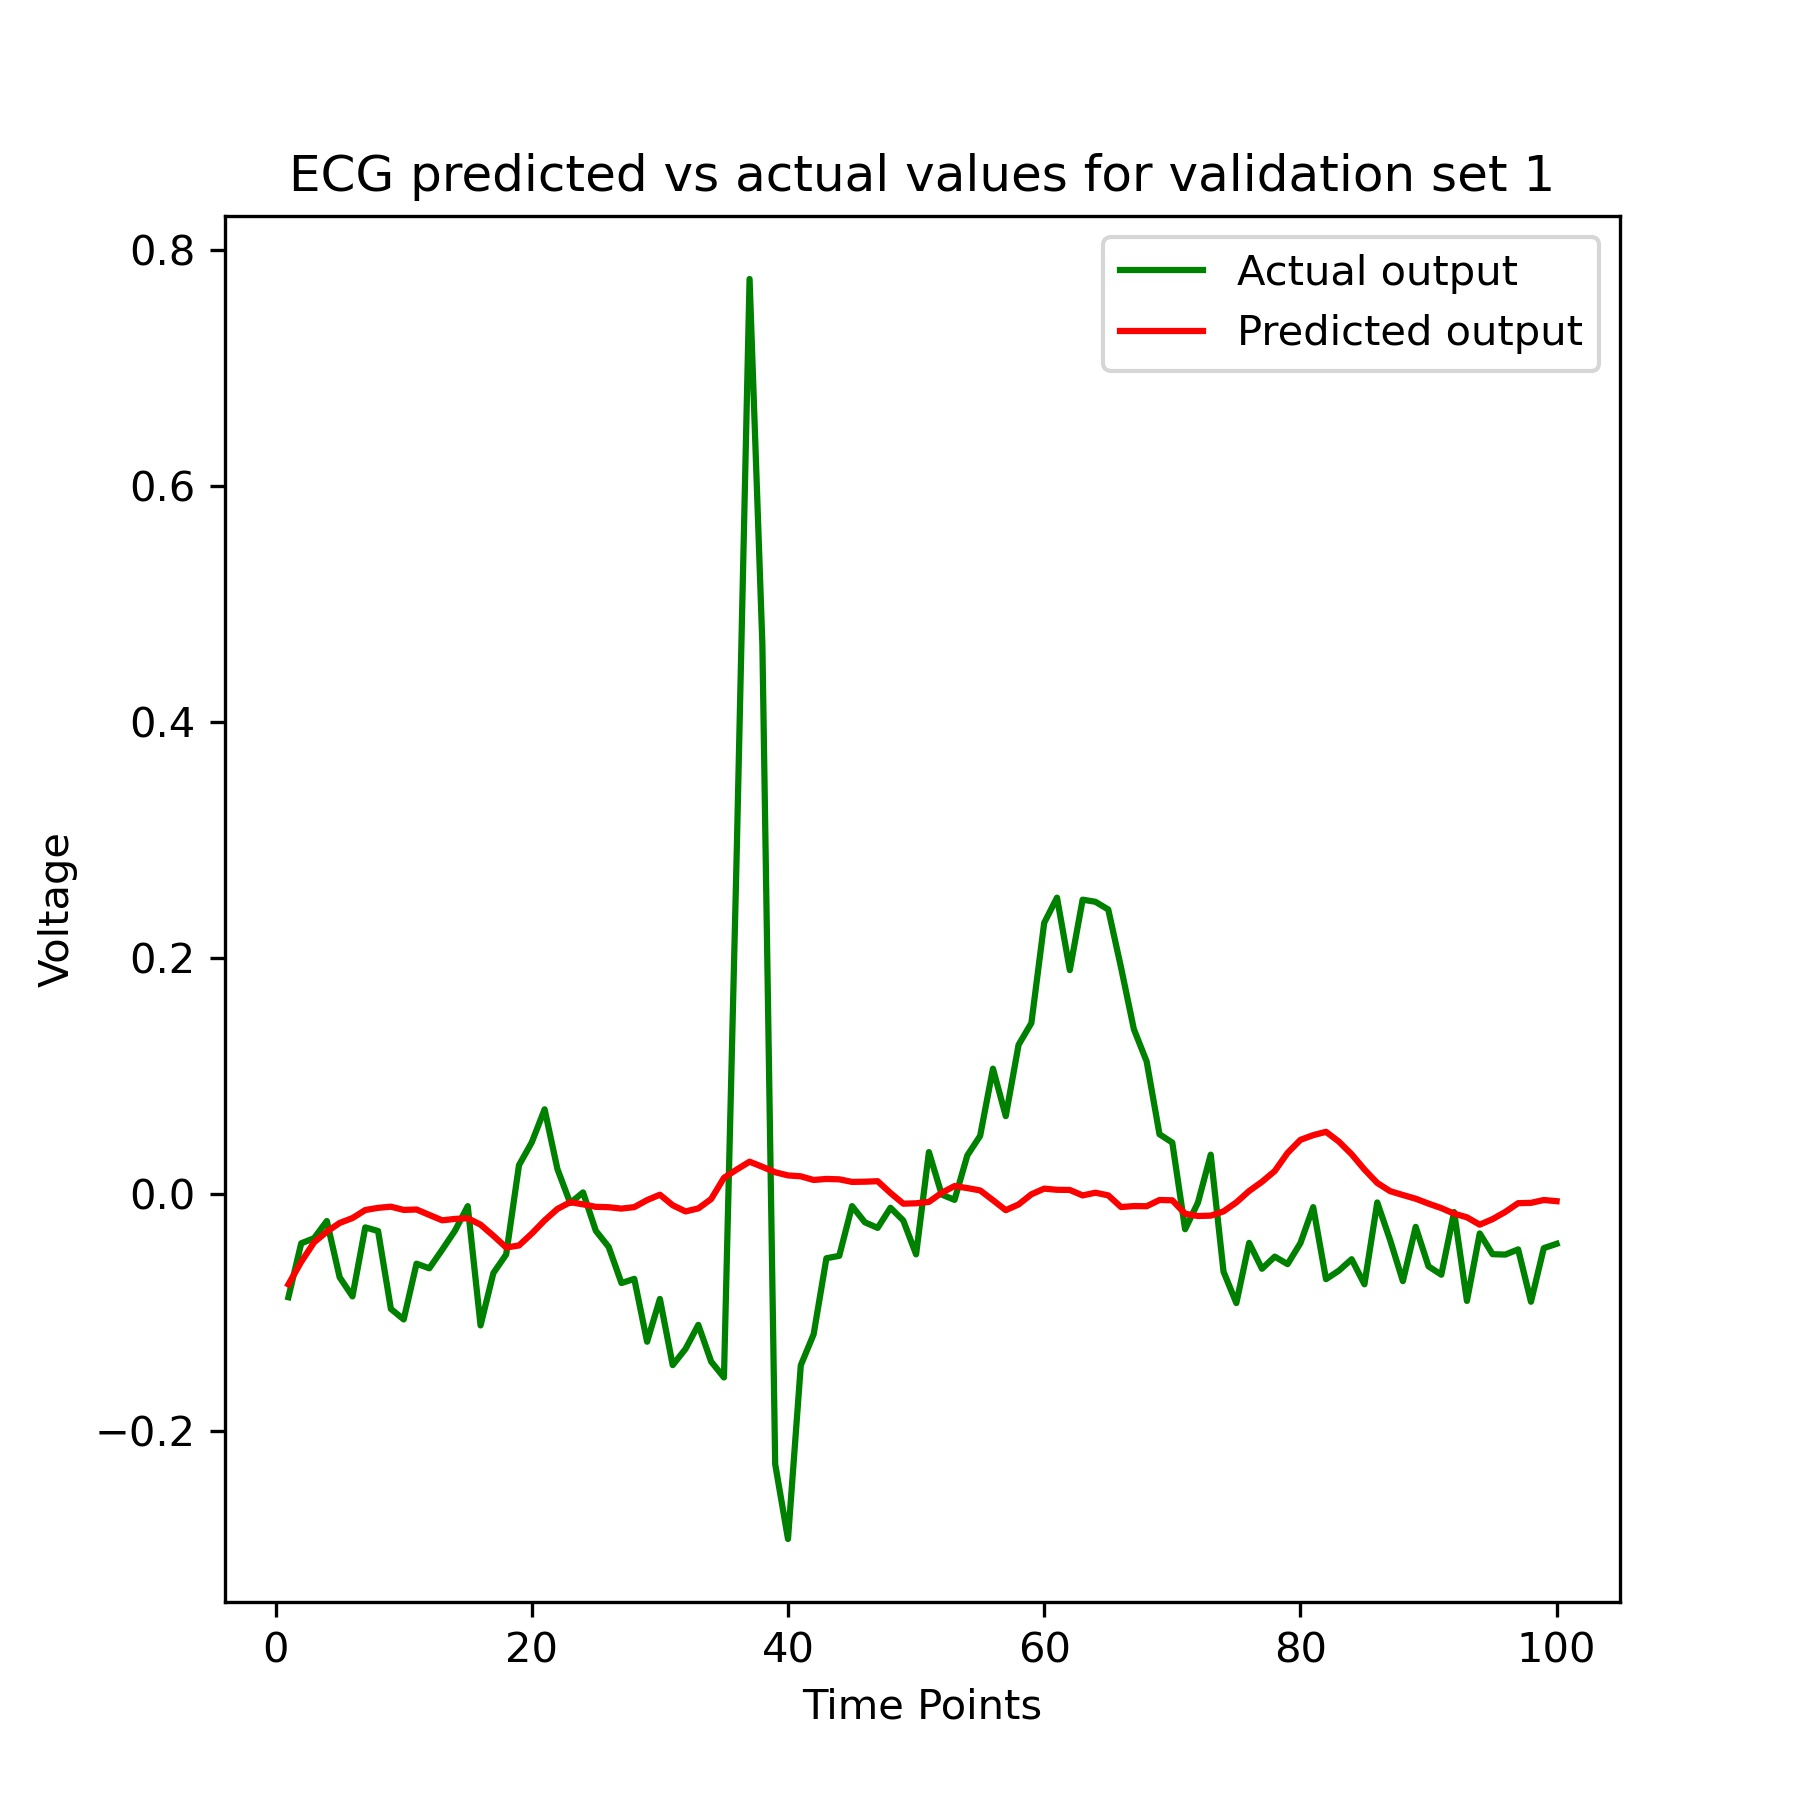
\includegraphics[width=\textwidth]{prediction_plot_1.jpg}
		\label{fig:val_pred_given_nn_1}
	\end{subfigure}
	\begin{subfigure}[b]{0.18\textwidth}
		\centering
		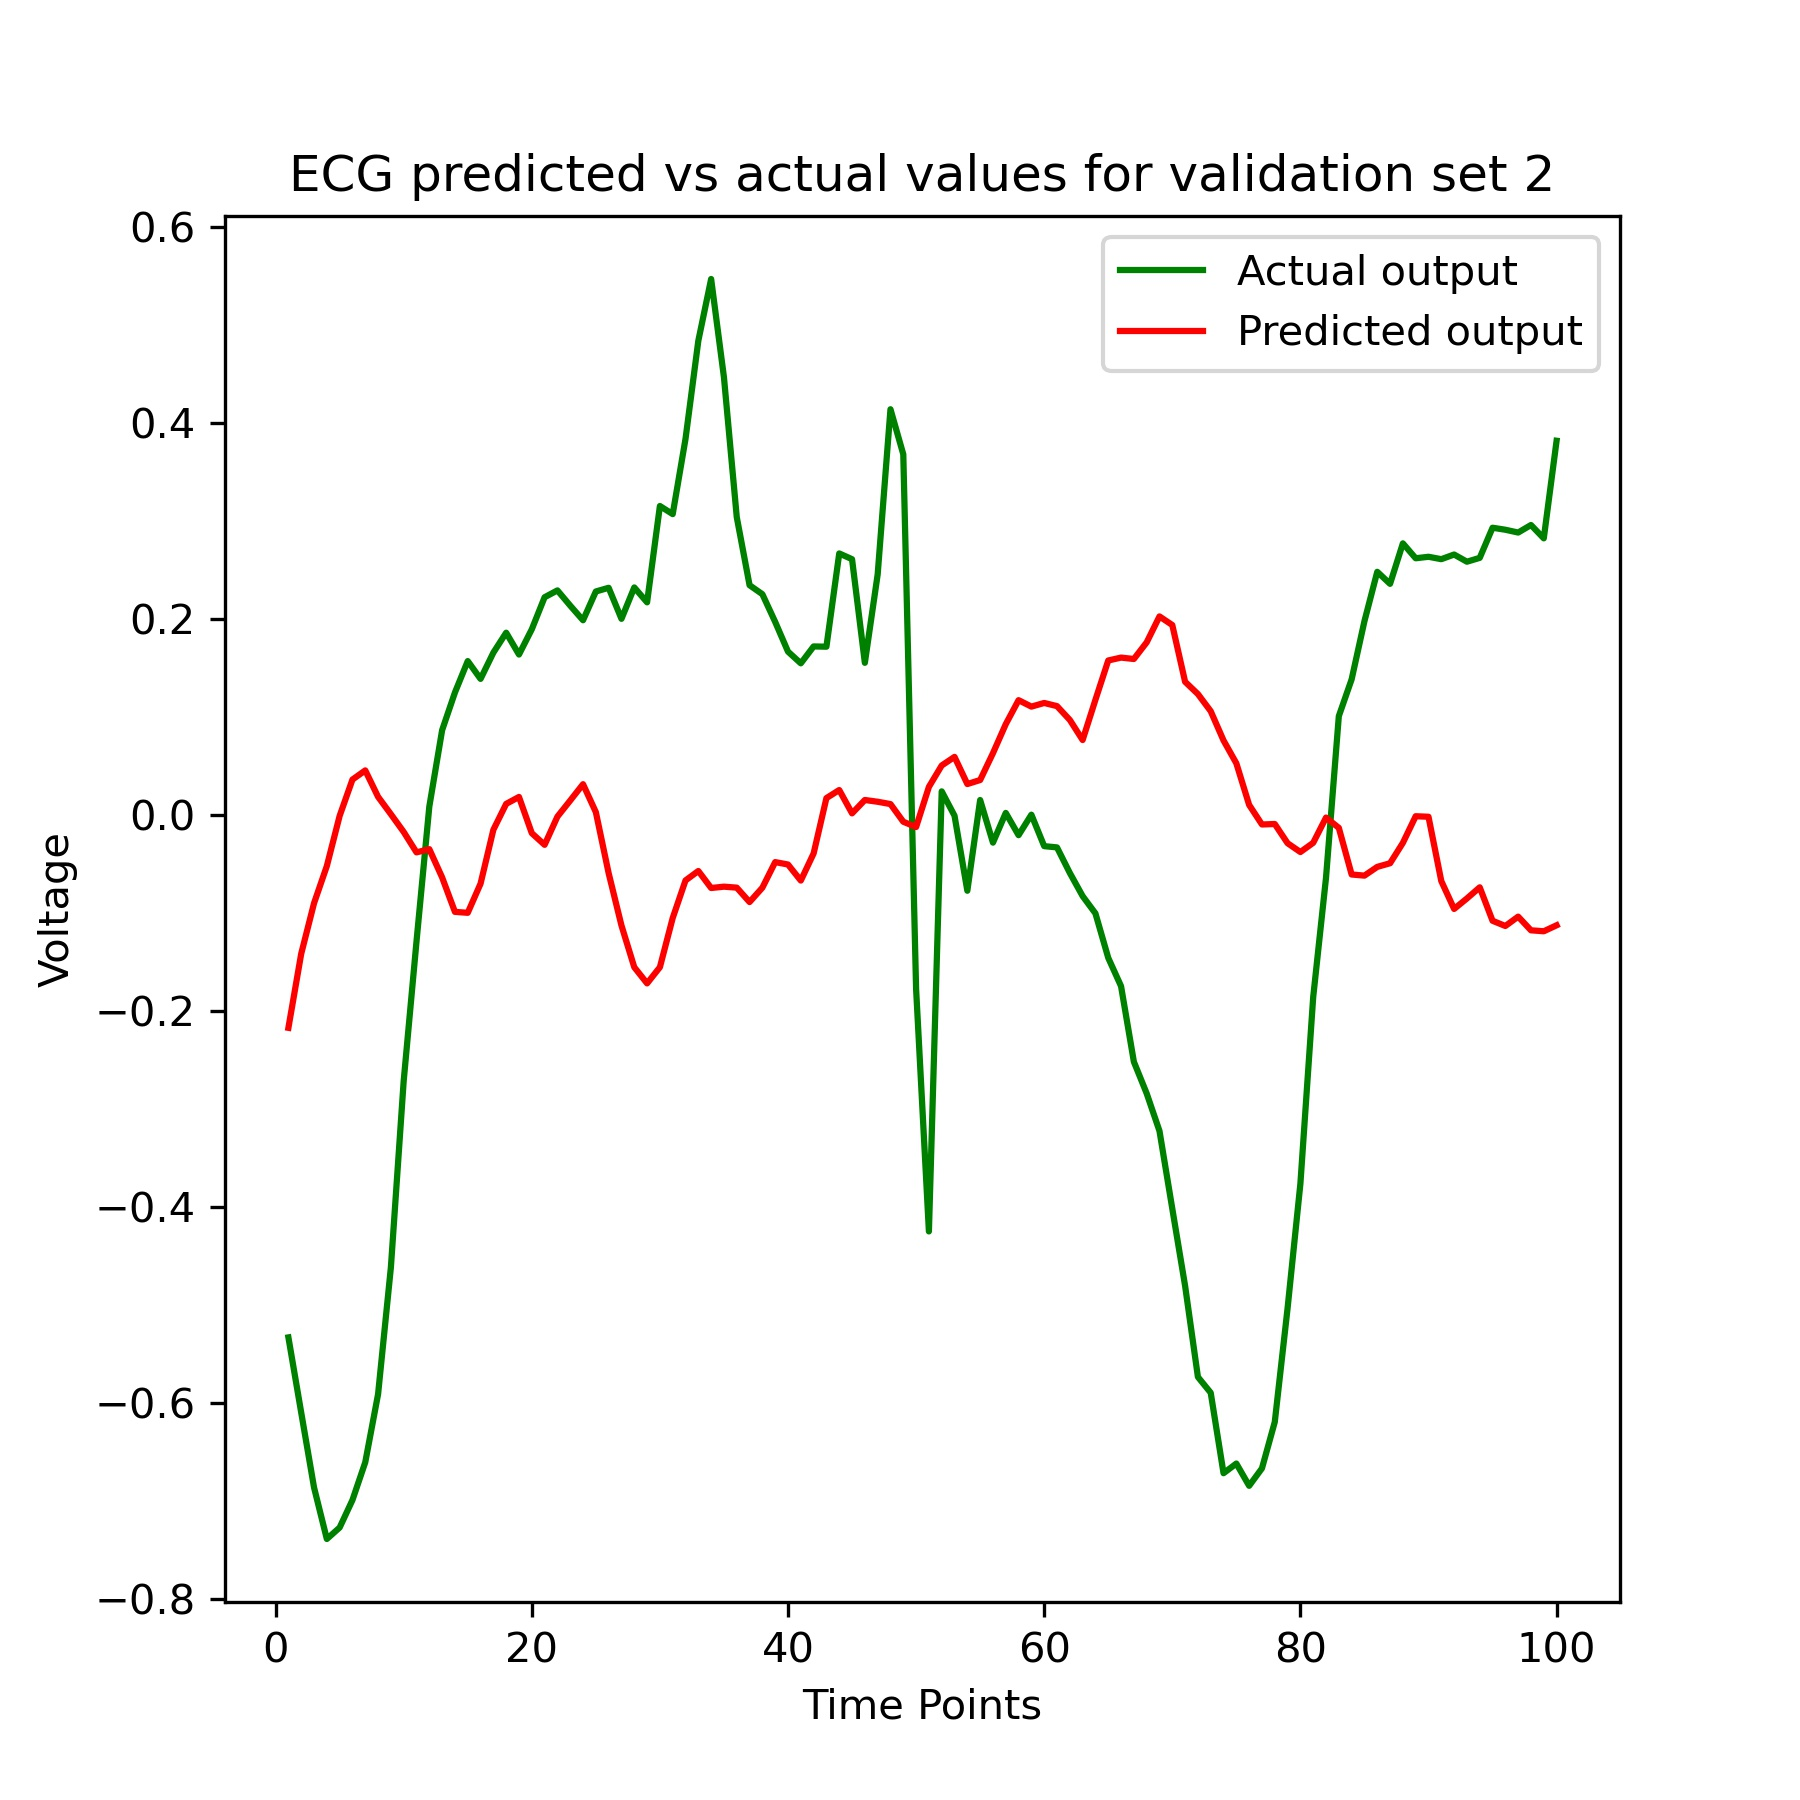
\includegraphics[width=\textwidth]{prediction_plot_2.jpg}
		\label{fig:val_pred_given_nn_2}
	\end{subfigure}
	\begin{subfigure}[b]{0.18\textwidth}
		\centering
		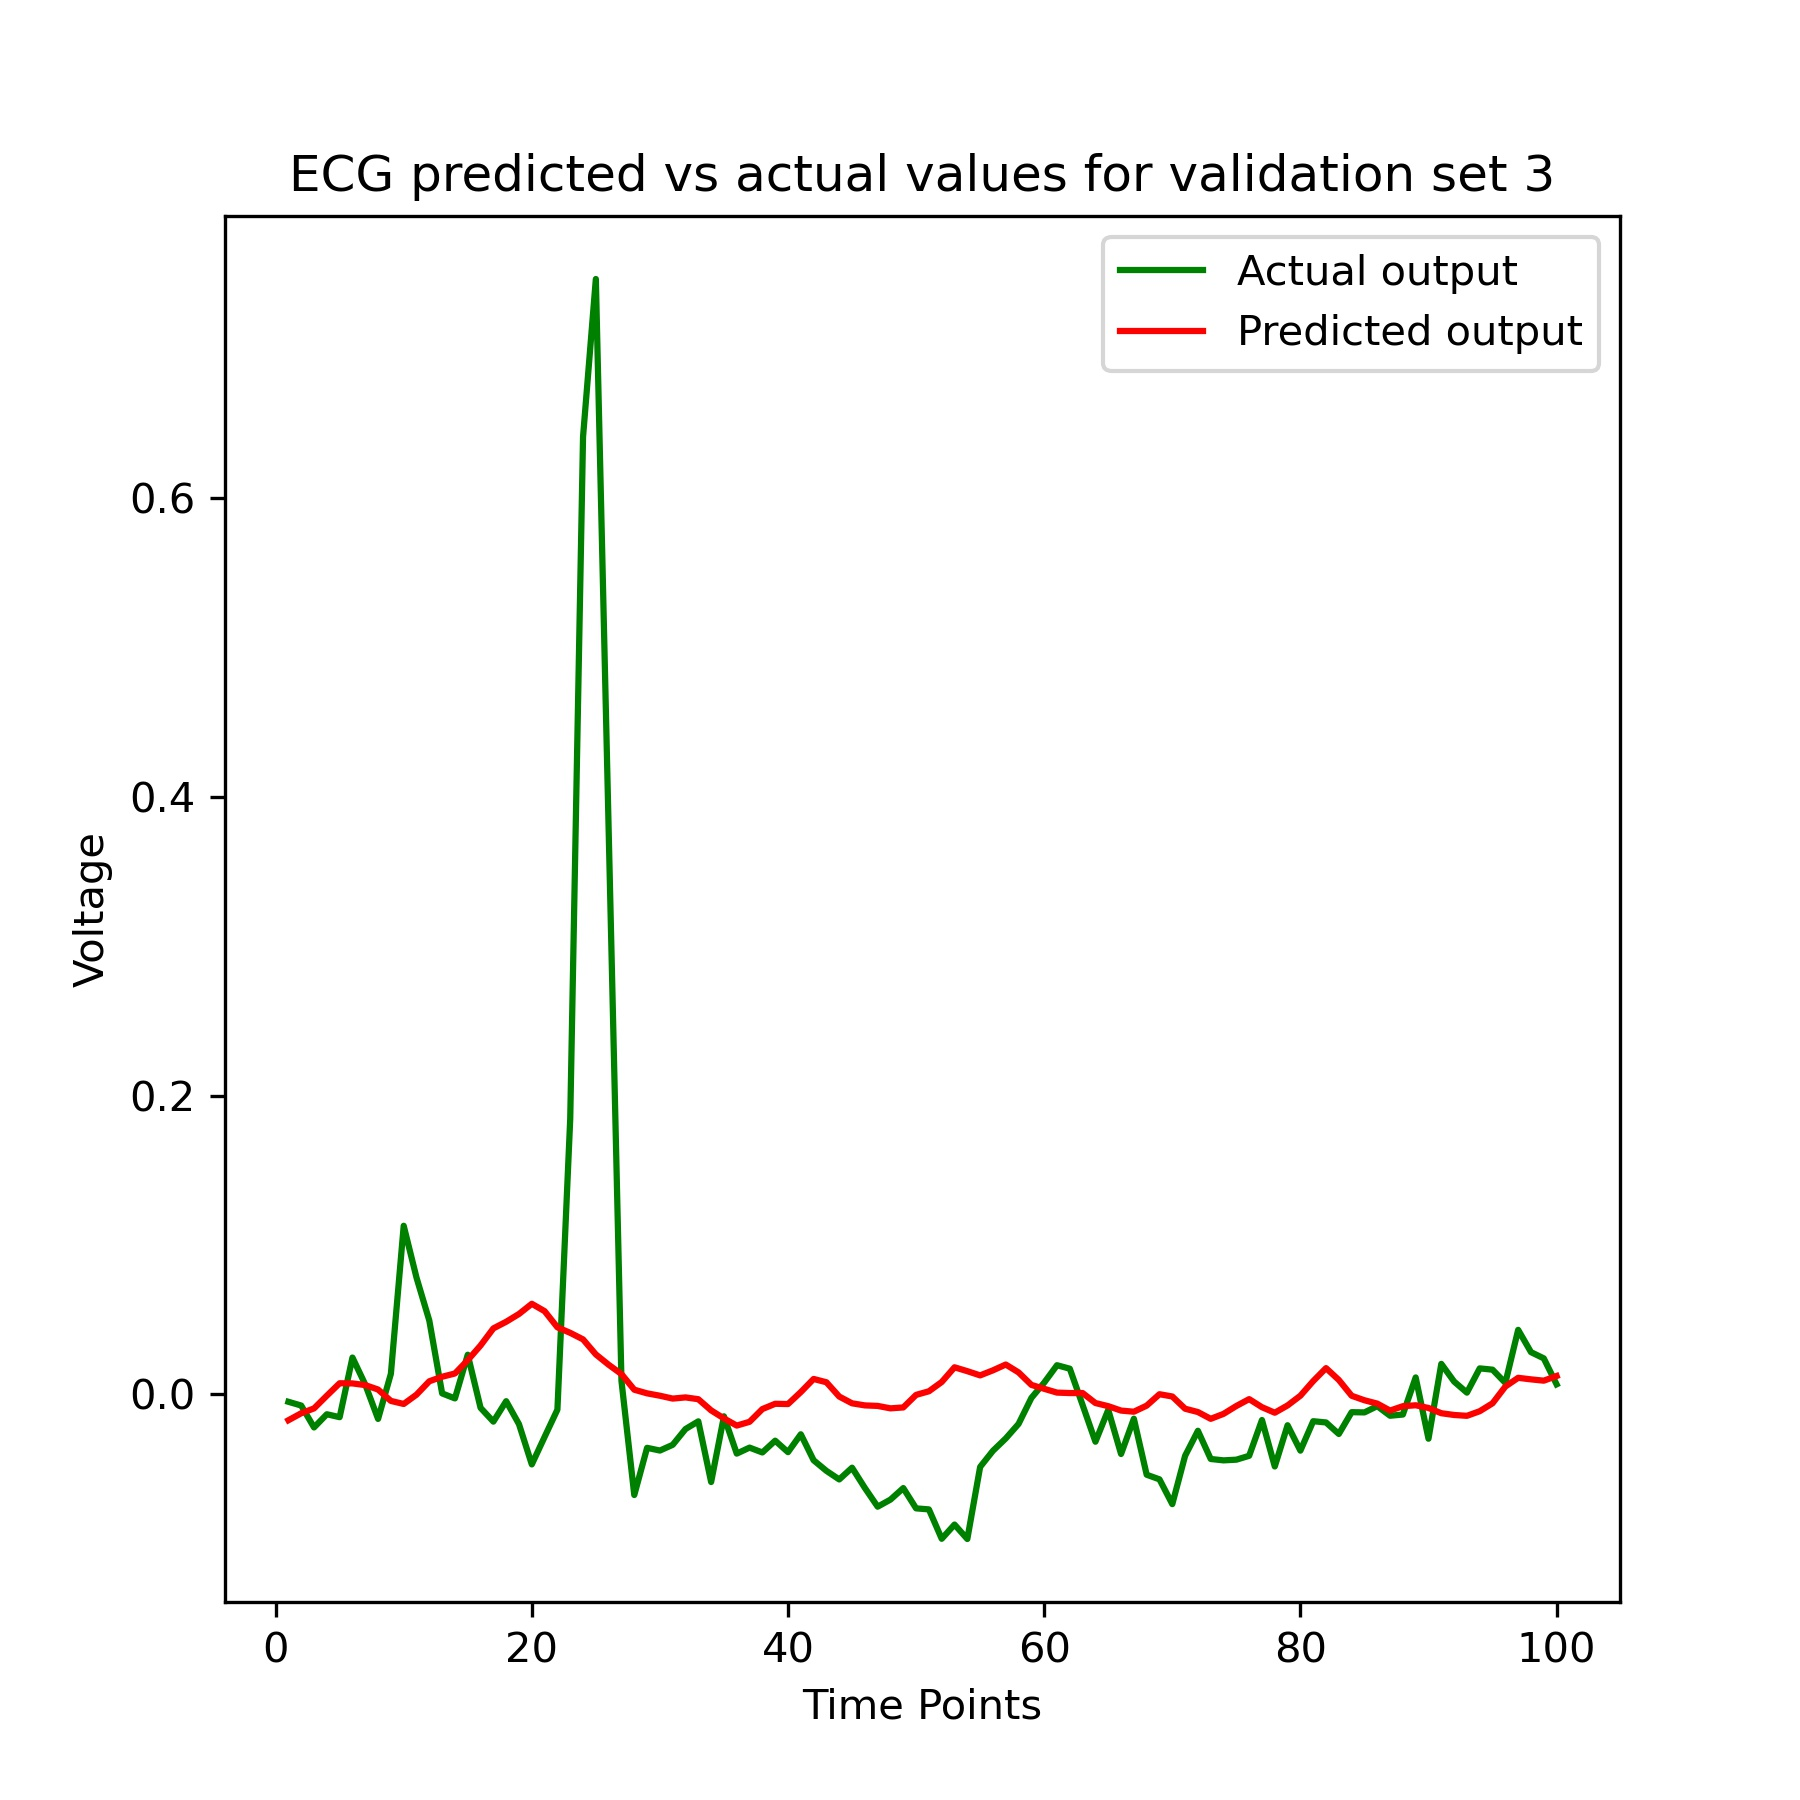
\includegraphics[width=\textwidth]{prediction_plot_3.jpg}
		\label{fig:val_pred_given_nn_3}
	\end{subfigure}
	\begin{subfigure}[b]{0.18\textwidth}
		\centering
		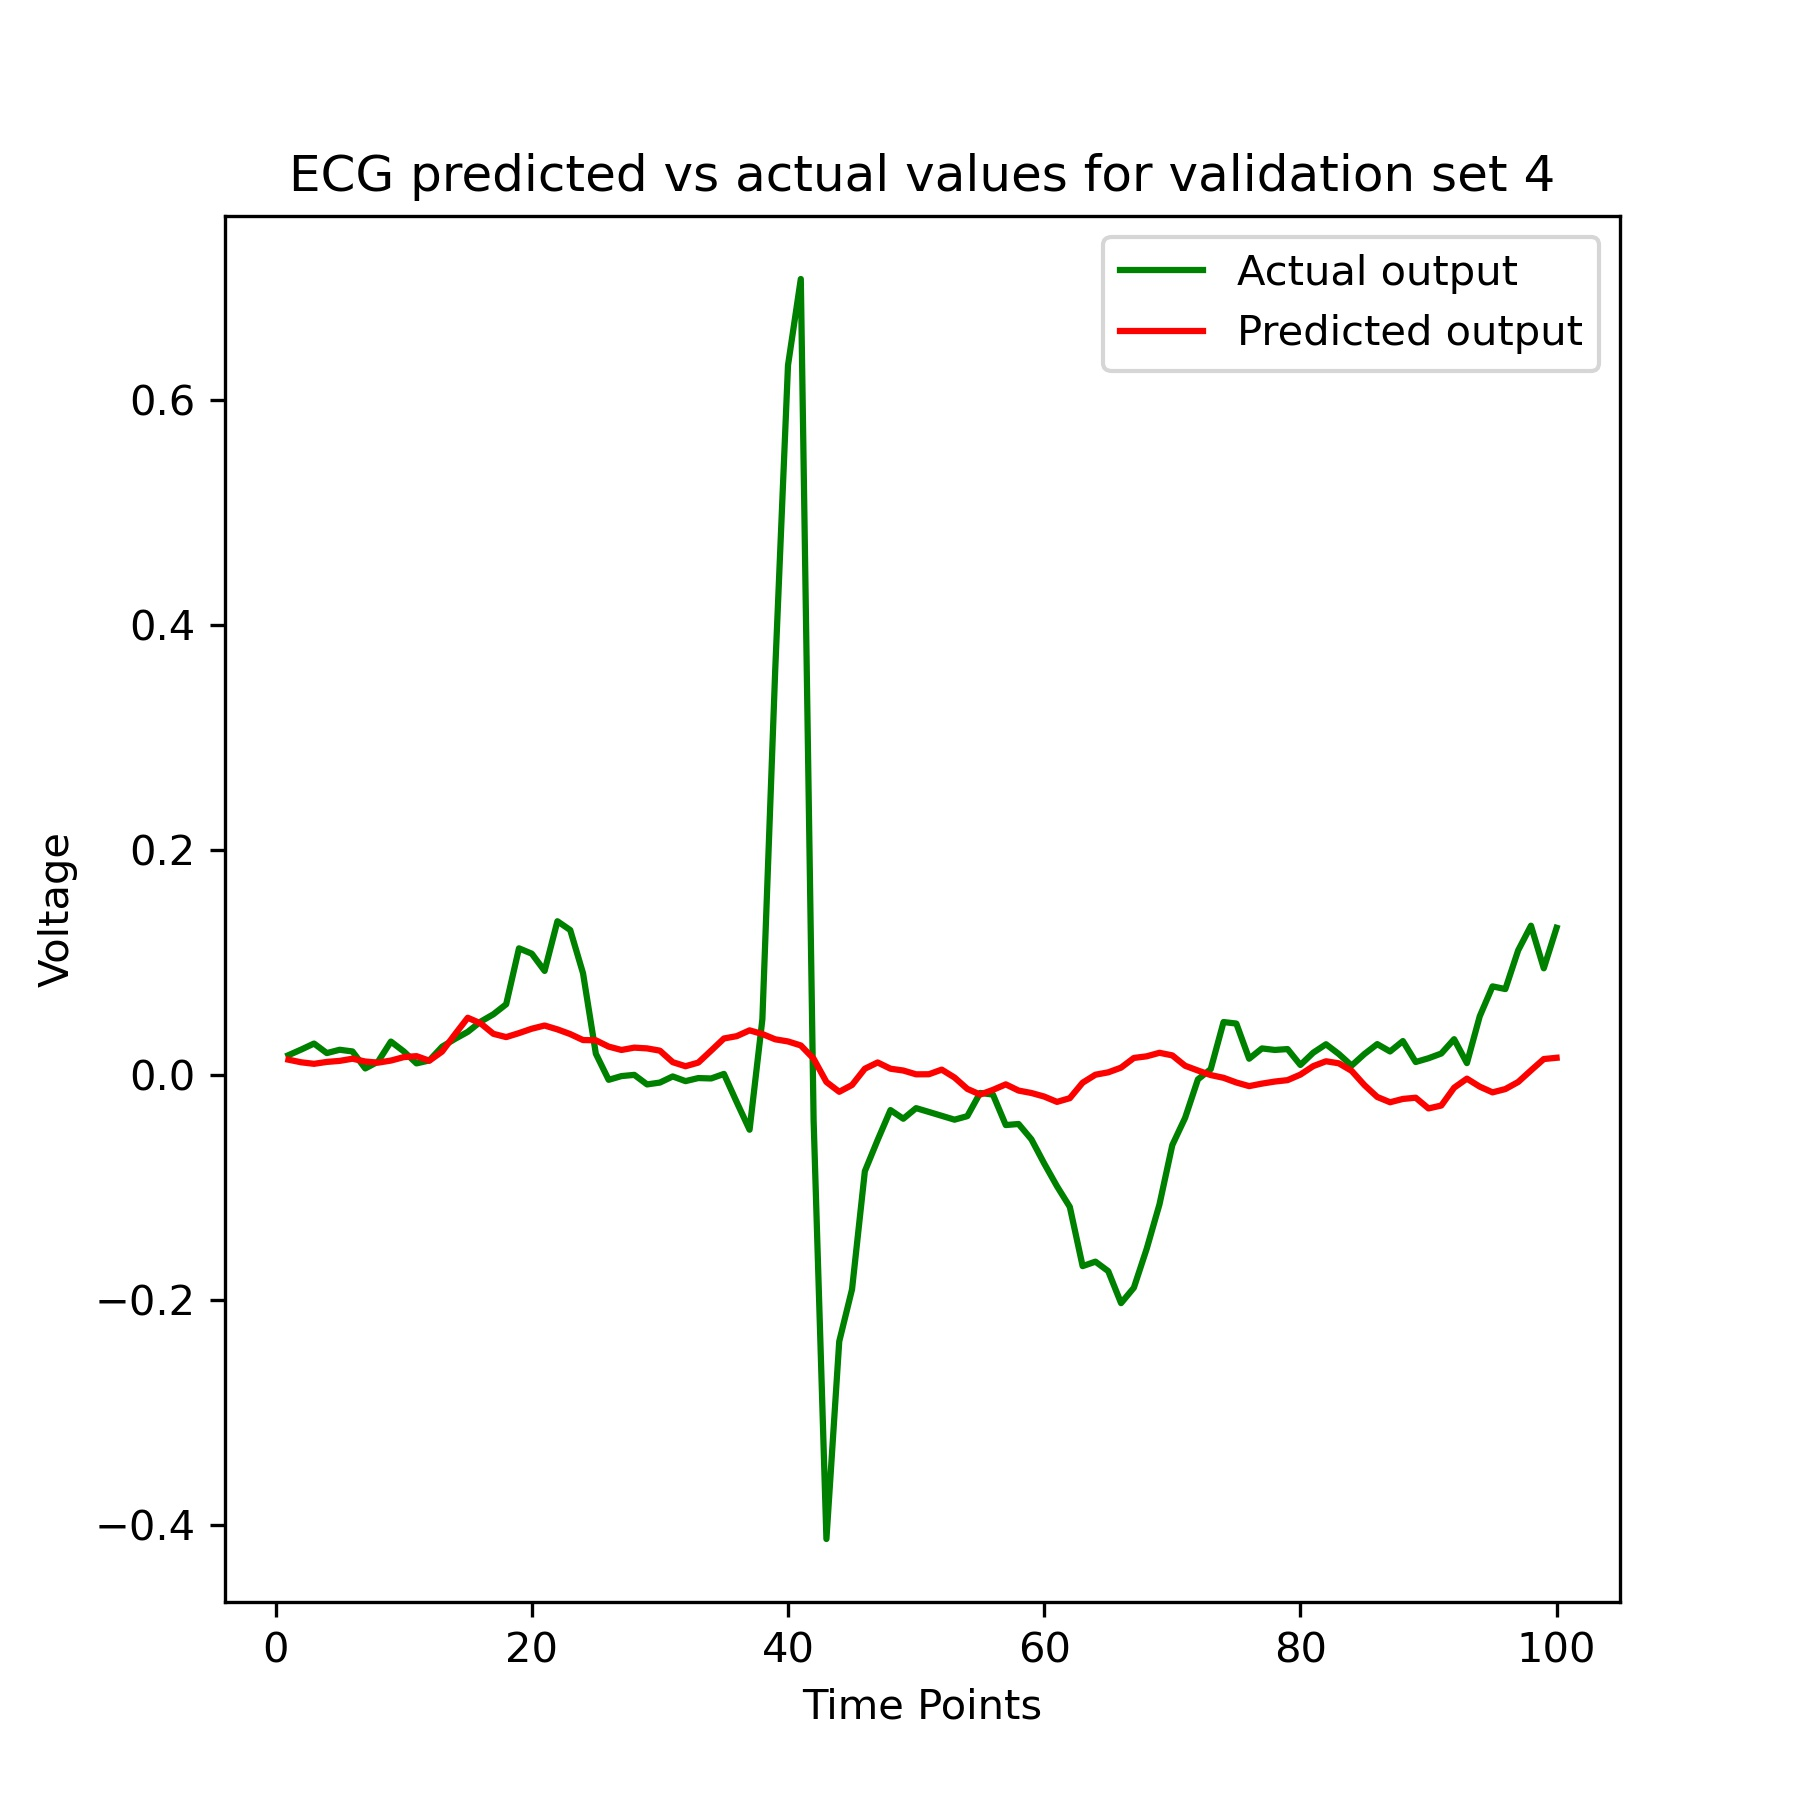
\includegraphics[width=\textwidth]{prediction_plot_4.jpg}
		\label{fig:val_pred_given_nn_3}
	\end{subfigure}
	\begin{subfigure}[b]{0.18\textwidth}
		\centering
		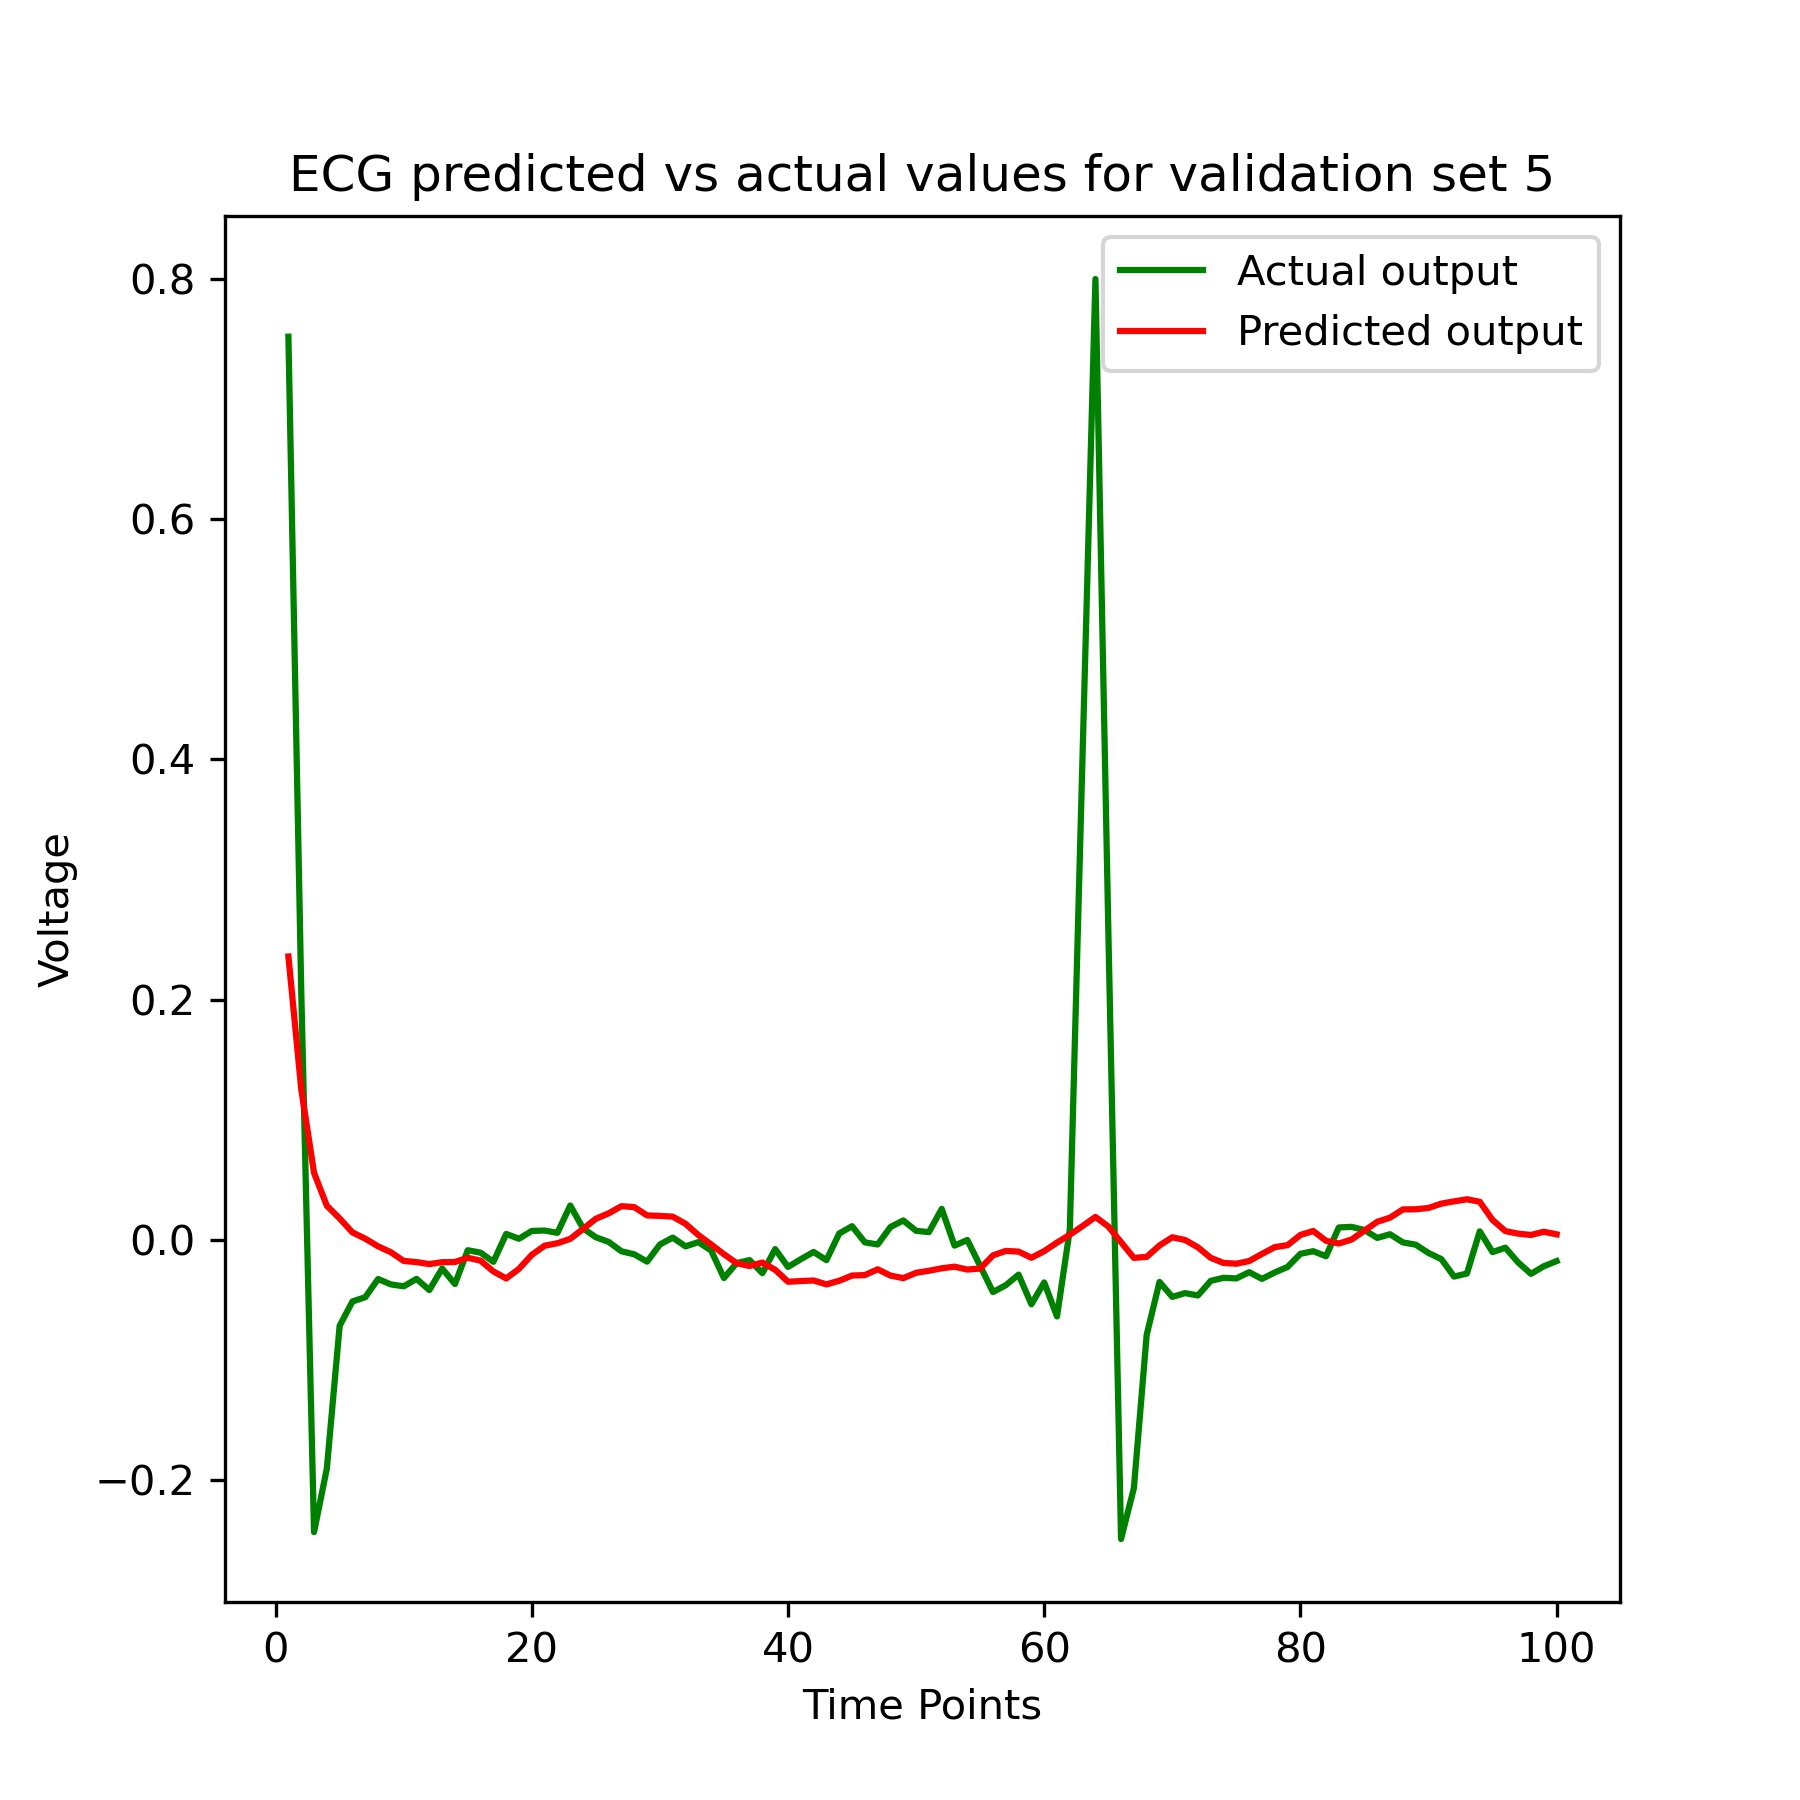
\includegraphics[width=\textwidth]{prediction_plot_5.jpg}
		\label{fig:val_pred_given_nn_3}
	\end{subfigure}
	\caption{Validation set outputs with their predictions for the first 5 validation sets using the given neural network architecture.}
	\label{fig:five_graphs}
\end{figure}

\begin{center}
	\line(1,0){450}
\end{center}

\textbf{3.a.}
I tried 3 model architectures - simple neural network (NN), CNN based model, and RNN based model with LSTM cells. CNN and RNN models have fully connected NN as the end layer. I shall describe below how I fine tuned both models: \\

$\mbf{Neural Network}$ \\

I used a 2 layer neural network with fixed size of hidden layer units (h1 > h2). I used Adam optimization algorithm and fine tuned the learning rate using a linear search process. Table \ref{tab:2layer_nn_adam_lr_effects} shows the best validation loss and number of epochs to achieve that loss for varying learning rates. Other parameters were kept fixed as $momentum=0.9$, $nesterov=False$. The learning rate curve for training and validation data can be seen in figure \ref{fig:lr_curve_2layer_nn_adam}. From these tests, we can see that 0.001 is a good choice for learning rate for Adam. I tried the same learning rate with RMSProp optimizer but the validation set loss was still 0.0200. \\

My second experiment with NN was to choose a one hidden layer model with Adam optimizer using fixed lr=0.001 and seeing effects of hidden layer size. The results are summarized in table \ref{tab:1layer_nn_adam_hunits_effects}. This indicates that NN architecture is not very good in capturing the details of the data set and adding more hidden units doesn't help in learning. Even 50 units achieves comparable performance. \\
 
\begin{table}[h!]
	\begin{center}
		\begin{tabular}{c|c|c|c|c|c} % <-- Alignments: 1st column left, 2nd middle and 3rd right, with vertical lines in between
			\textbf{Learning rate} & 0.0001 & \bf0.001 & 0.01 & 0.1 & 1\\
			\hline
			\textbf{Best validation loss} & 0.0199 & 0.0200 & 0.0206 & 0.0206 & 0.0222\\
			\hline
			\textbf{num of epochs} & 279 & 51 & 115 & 273 & 1
		\end{tabular}
		\caption{Effect of learning rate on final validation loss for 2 layer NN model.}
		\label{tab:2layer_nn_adam_lr_effects}
	\end{center}
\end{table}

\begin{figure}
	\centering
	\begin{subfigure}[b]{0.18\textwidth}
		\centering
		\includegraphics[width=\textwidth]{train_val_loss_nn_{'hl_1_units': 500, 'hl_2_units': 200, 'learning_rate': 0.0001, 'momentum': 0.9, 'nesterov': False, 'optimizer': <Optimizer.ADAM: 1>}.jpg}
		\caption{lr=0.0001}
		\label{fig:lr_curve_2layer_nn_adam_1}
	\end{subfigure}
	\begin{subfigure}[b]{0.18\textwidth}
		\centering
		\includegraphics[width=\textwidth]{train_val_loss_nn_{'hl_1_units': 500, 'hl_2_units': 200, 'learning_rate': 0.001, 'momentum': 0.9, 'nesterov': False, 'optimizer': <Optimizer.ADAM: 1>}.jpg}
		\caption{lr=0.001}
		\label{fig:lr_curve_2layer_nn_adam_2}
	\end{subfigure}
	\begin{subfigure}[b]{0.18\textwidth}
		\centering
		\includegraphics[width=\textwidth]{train_val_loss_nn_{'hl_1_units': 500, 'hl_2_units': 200, 'learning_rate': 0.01, 'momentum': 0.9, 'nesterov': False, 'optimizer': <Optimizer.ADAM: 1>}.jpg}
		\caption{lr=0.01}
		\label{fig:lr_curve_2layer_nn_adam_3}
	\end{subfigure}
	\begin{subfigure}[b]{0.18\textwidth}
		\centering
		\includegraphics[width=\textwidth]{train_val_loss_nn_{'hl_1_units': 500, 'hl_2_units': 200, 'learning_rate': 0.1, 'momentum': 0.9, 'nesterov': False, 'optimizer': <Optimizer.ADAM: 1>}.jpg}
		\caption{lr=0.1}
		\label{fig:lr_curve_2layer_nn_adam_4}
	\end{subfigure}
	\begin{subfigure}[b]{0.18\textwidth}
		\centering
		\includegraphics[width=\textwidth]{train_val_loss_nn_{'hl_1_units': 500, 'hl_2_units': 200, 'learning_rate': 1.0, 'momentum': 0.9, 'nesterov': False, 'optimizer': <Optimizer.ADAM: 1>}.jpg}
		\caption{lr=1.0}
		\label{fig:lr_curve_2layer_nn_adam_5}
	\end{subfigure}	
	\caption{Learning rate curve for a 2 hiddel layer NN model with Adam optimizer for varying learning\_rate values.}
	\label{fig:lr_curve_2layer_nn_adam}
\end{figure}

\begin{table}[h!]
	\begin{center}
		\begin{tabular}{c|c|c|c|c|c} % <-- Alignments: 1st column left, 2nd middle and 3rd right, with vertical lines in between
			\textbf{Hidden layer units} & 50 & 100 & 300 & 400 & \bf500\\
			\hline
			\textbf{Best validation loss} & 0.0205 & 0.0206 & 0.0204 & 0.0204 & 0.0203\\
			\hline
			\textbf{num of epochs} & 118 & 63 & 55 & 54 & 51
		\end{tabular}
		\caption{Effects of number of hidden units on learning rate for 1 layer NN model.}
		\label{tab:1layer_nn_adam_hunits_effects}
	\end{center}
\end{table}

$\mbf{CNN}$ \\

CNN models have lots of hyperparamters to choose from. I selected an architecture having 2 blocks of Conv-ReLU-MaxPool followed by a linear layer. The hyperparameters to tune here were number of filters (out\_channels), filter size (kernel\_size) and maxpool size for each block. Optimizer was fixed to Adam with lr=0.001. In first test, I tried different number of filters keeping other parameters fixed. The validation set loss is summarized in table \ref{tab:2block_cnn_num_filter_effects}.

In next test, I fixed the number of filters to 10 and changed kernel size keeping the stride fixed to 1. Results are in table \ref{tab:2block_cnn_kernel_size_effects}. Another test was done to test the effects of max-pooling by keeping filter size as 10 and kernel size as 20. Results are in table \ref{tab:2block_cnn_maxpool_size_effects}. As you can see, in each successive test, I used the optimum value optained from the previous tests and kept those constant.

\begin{table}
	\parbox{.45\linewidth}{
		\centering
		\begin{tabular}{c|c|c|c}
			\textbf{Number of filters} & 4 & \bf10 & 20\\
			\hline
			\textbf{Best validation loss} & 0.0206 & 0.0206 & 0.0206\\
			\hline
			\textbf{Num of epochs} & 43 & 24 & 45
		\end{tabular}
		\caption{Effects of filter size on 2 block CNN model. Same filter size is used for both blocks.}
		\label{tab:2block_cnn_num_filter_effects}
	}
	\hfill
	\parbox{.45\linewidth}{
		\centering
		\begin{tabular}{c|c|c|c} % <-- Alignments: 1st column left, 2nd middle and 3rd right, with vertical lines in between
			\textbf{Kernel size} & 5 & \bf10 & 20\\
			\hline
			\textbf{Best validation loss} & 0.0207 & 0.0206 & 0.0206\\
			\hline
			\textbf{Num of epochs} & 42 & 20 & 11
		\end{tabular}
		\caption{Effects of kernel size on 2 block CNN model. Same kernel size is used for both blocks.}
		\label{tab:2block_cnn_kernel_size_effects}
	}
\end{table}

\begin{table}[h!]
	\begin{center}
		\begin{tabular}{c|c|c|c} % <-- Alignments: 1st column left, 2nd middle and 3rd right, with vertical lines in between
			\textbf{Maxpool size} & \bf3 & 5 & 8\\
			\hline
			\textbf{Best validation loss} & 0.0207 & 0.0206 & 0.0206\\
			\hline
			\textbf{Num of epochs} & 21 & 30 & 24
		\end{tabular}
		\caption{Effects of Maxpool size on 2 block CNN model. Same maxpool size is used for both blocks.}
		\label{tab:2block_cnn_maxpool_size_effects}
	\end{center}
\end{table}

$\mbf{RNN}$ \\

There are different varieties of RNN architectures that can be chosen. For this task, I decided to use multi-layer RNN model with LSTM cells as the first layer and fully connected NN at the end. LSTM is popular for time sequence estimation tasks and combined with RNN architecture, it can work well. The hyperparameters are number of hidden units and number of RNN layers. I am fixing the linear layer to 1 as making it 2 did not provide improved performance in a separate test.

In the first test, I fixed the hidden layers to 1 and tried multiple values of hidden units. Results are in table \ref{tab:rnn_1hl_hidden_units_effects}. In second test, I fixed the hidden layers to 2 and tried same set of hidden unit values. Results are in table \ref{tab:rnn_2hl_hidden_units_effects}. \\

\begin{table}[h!]
	\begin{center}
		\begin{tabular}{c|c|c|c|c} % <-- Alignments: 1st column left, 2nd middle and 3rd right, with vertical lines in between
			\textbf{Hidden layer units} & 200 & \bf300 & 400 & 500\\
			\hline
			\textbf{Best validation loss} & 0.0205 & 0.0204 & 0.0204 & 0.0204\\
			\hline
			\textbf{Num of epochs} & 91 & 100 & 76 & 90
		\end{tabular}
		\caption{Effects of hidden layer size RNN model with LSTM cells.}
		\label{tab:rnn_1hl_hidden_units_effects}
	\end{center}
\end{table}

\begin{table}[h!]
	\begin{center}
		\begin{tabular}{c|c|c|c|c} % <-- Alignments: 1st column left, 2nd middle and 3rd right, with vertical lines in between
			\textbf{Hidden layer units} & 200 & \bf300 & 400 & 500\\
			\hline
			\textbf{Best validation loss} & 0.0202 & 0.0202 & 0.0203 & 0.0203\\
			\hline
			\textbf{Num of epochs} & 118 & 113 & 110 & 102
		\end{tabular}
		\caption{Effects of hidden layer size RNN model with LSTM cells.}
		\label{tab:rnn_2hl_hidden_units_effects}
	\end{center}
\end{table}

\textbf{3.b.}
To select the best model, I compared three different architectures (NN, CNN, RNN with LSTM) and tuned their hyperparameters. The strategy to select their hyperparameters is discussed in part 3.a. Models are compared based on validation set loss, and training is done by keeping batch size as total size of data. Since the number of examples is less and models were overfitting easily, I did not go with mini batch approach.

From all the experimentation, I notice that all the models have almost similar performance. A statistical test can better compare the models, but looking at the prediction graphs, no model has been able to learn the spikes well.

For each table, I have made bold the best hyperparameter value. The best model is a 2 layer NN with Adam optimizer. \\

\textbf{3.c.} The architecture for the best model is in figure \ref{fig:best_nn}. It is implemented using sequential container in pytorch. It is described as:

\begin{figure}[h]
	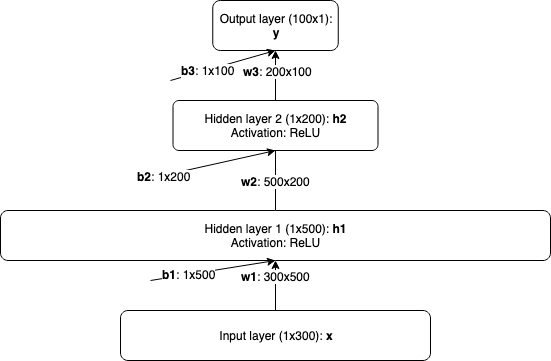
\includegraphics[scale=0.5]{best_nn.png}
	\centering
	\caption{Architecture diagram for the best model: a multi layer neural network.}
	\label{fig:best_nn}
\end{figure}

\textbf{3.d.} The best neural network model selection technique has already been explained in section 3.a. above. The hyperparameters for this model were number of layers, number of hidden units in a layer, optimizer, and learning rate. Number of hidden layers was chosen by doing experiments for 1 and 2 hidden layers and picking the best according to validation set loss. Adam was chosen as the default optimizer but its learning rate was chosen using a 1D grid search approach. Momemtum was kept as the default because conversion rate was not seen as a problem after tuning the learning rate. \\

\textbf{3.e.} The line plots are in figure \ref{fig:best_nn_val_pred}. \\

\begin{figure}
	\centering
	\begin{subfigure}[b]{0.18\textwidth}
		\centering
		\includegraphics[width=\textwidth]{prediction_plot_nn_{'hl_1_units': 500, 'hl_2_units': 200, 'learning_rate': 0.001, 'momentum': 0.9, 'nesterov': False, 'optimizer': <Optimizer.ADAM: 1>}val_1.jpg}
		\label{fig:best_nn_val_pred_1}
	\end{subfigure}
	\begin{subfigure}[b]{0.18\textwidth}
		\centering
		\includegraphics[width=\textwidth]{prediction_plot_nn_{'hl_1_units': 500, 'hl_2_units': 200, 'learning_rate': 0.001, 'momentum': 0.9, 'nesterov': False, 'optimizer': <Optimizer.ADAM: 1>}val_2.jpg}
		\label{fig:best_nn_val_pred_2}
	\end{subfigure}
	\begin{subfigure}[b]{0.18\textwidth}
		\centering
		\includegraphics[width=\textwidth]{prediction_plot_nn_{'hl_1_units': 500, 'hl_2_units': 200, 'learning_rate': 0.001, 'momentum': 0.9, 'nesterov': False, 'optimizer': <Optimizer.ADAM: 1>}val_3.jpg}
		\label{fig:best_nn_val_pred_3}
	\end{subfigure}
	\begin{subfigure}[b]{0.18\textwidth}
		\centering
		\includegraphics[width=\textwidth]{prediction_plot_nn_{'hl_1_units': 500, 'hl_2_units': 200, 'learning_rate': 0.001, 'momentum': 0.9, 'nesterov': False, 'optimizer': <Optimizer.ADAM: 1>}val_4.jpg}
		\label{fig:best_nn_val_pred_4}
	\end{subfigure}
	\begin{subfigure}[b]{0.18\textwidth}
		\centering
		\includegraphics[width=\textwidth]{prediction_plot_nn_{'hl_1_units': 500, 'hl_2_units': 200, 'learning_rate': 0.001, 'momentum': 0.9, 'nesterov': False, 'optimizer': <Optimizer.ADAM: 1>}val_5.jpg}
		\label{fig:best_nn_val_pred_5}
	\end{subfigure}	
	\caption{Validation data output and predictions for the first 5 sets using the best model.}
	\label{fig:best_nn_val_pred}
\end{figure}

\textbf{3.f.} For this task, I retrained the model using both validation and training data so that the data set size increases.

\end{document}
